\documentclass{beamer}
\usepackage[utf8]{inputenc}
\usepackage[T1]{fontenc}

\setbeamerfont{title}{size=\LARGE}

\title{Bash I}
\author{Eliška Jégrová}
\date{30. 09. 2025}

% pro obrázky a kreslení
\usepackage{tikz}
\usetikzlibrary{positioning}
\usepackage{graphicx}
\usepackage{datetime}
\usepackage{svg}
\usepackage{listings}


% vlastní příkaz pro tildy
\newcommand{\ts}{\raisebox{-0.25em}{\textasciitilde}}

\begin{document}

  \frame{\titlepage}

  \begin{frame}{Obsah}
    \tableofcontents
  \end{frame}

\section{Úvod do Bashe}
\begin{frame}{Úvod do Bashe}
  \begin{columns}[c]
    \column{0.55\textwidth}
    \textbf{Jak funguje operační systém:}
    \begin{itemize}
      \item \textbf{Jádro (kernel)} – spravuje hardware, procesy, paměť, disky.
      \item \textbf{Shell} – prostředník mezi uživatelem a jádrem, interpretuje příkazy.
      \item \textbf{Programy} – aplikace, které používáme (editor, prohlížeč, skripty).
      \item Bash = jeden z nejrozšířenějších shellů.
    \end{itemize}

    \vspace{0.5em}
    \textit{Uživatel $\rightarrow$ Shell $\rightarrow$ Jádro $\rightarrow$ Hardware}

    \column{0.45\textwidth}
    \centering
    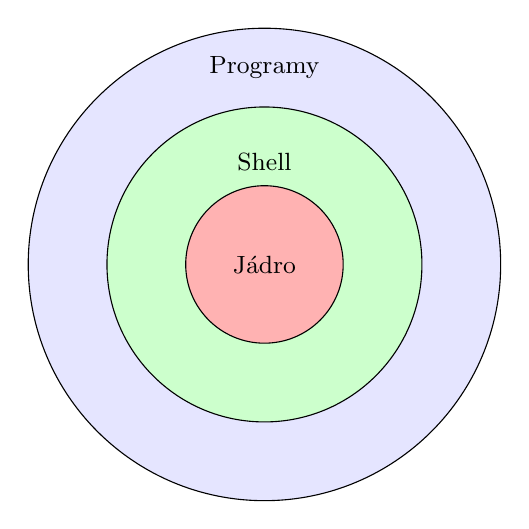
\begin{tikzpicture}
      % Vnější kruh - Programy
      \draw[fill=blue!10] (0,0) circle (3cm);
      \node at (0,2.5) {\small Programy};

      % Prostřední kruh - Shell
      \draw[fill=green!20] (0,0) circle (2cm);
      \node at (0,1.3) {\small Shell};

      % Vnitřní kruh - Jádro
      \draw[fill=red!30] (0,0) circle (1cm);
      \node at (0,0) {\small Jádro};
    \end{tikzpicture}
    \vspace{0.5em}
  \end{columns}
\end{frame}

\begin{frame}{Proč terminál / shell?}
  \begin{columns}[c]
    \column{0.55\textwidth}
    \begin{itemize}
      \item Rychlejší práce oproti klikání v GUI
      \item Možnost automatizace a skriptování
      \item Nezbytný pro práci na serverech (bez grafiky)
      \item Jednoduše předám výstup nebo chybovou hlášku ostatním
    \end{itemize}


    \column{0.45\textwidth}
    \centering
    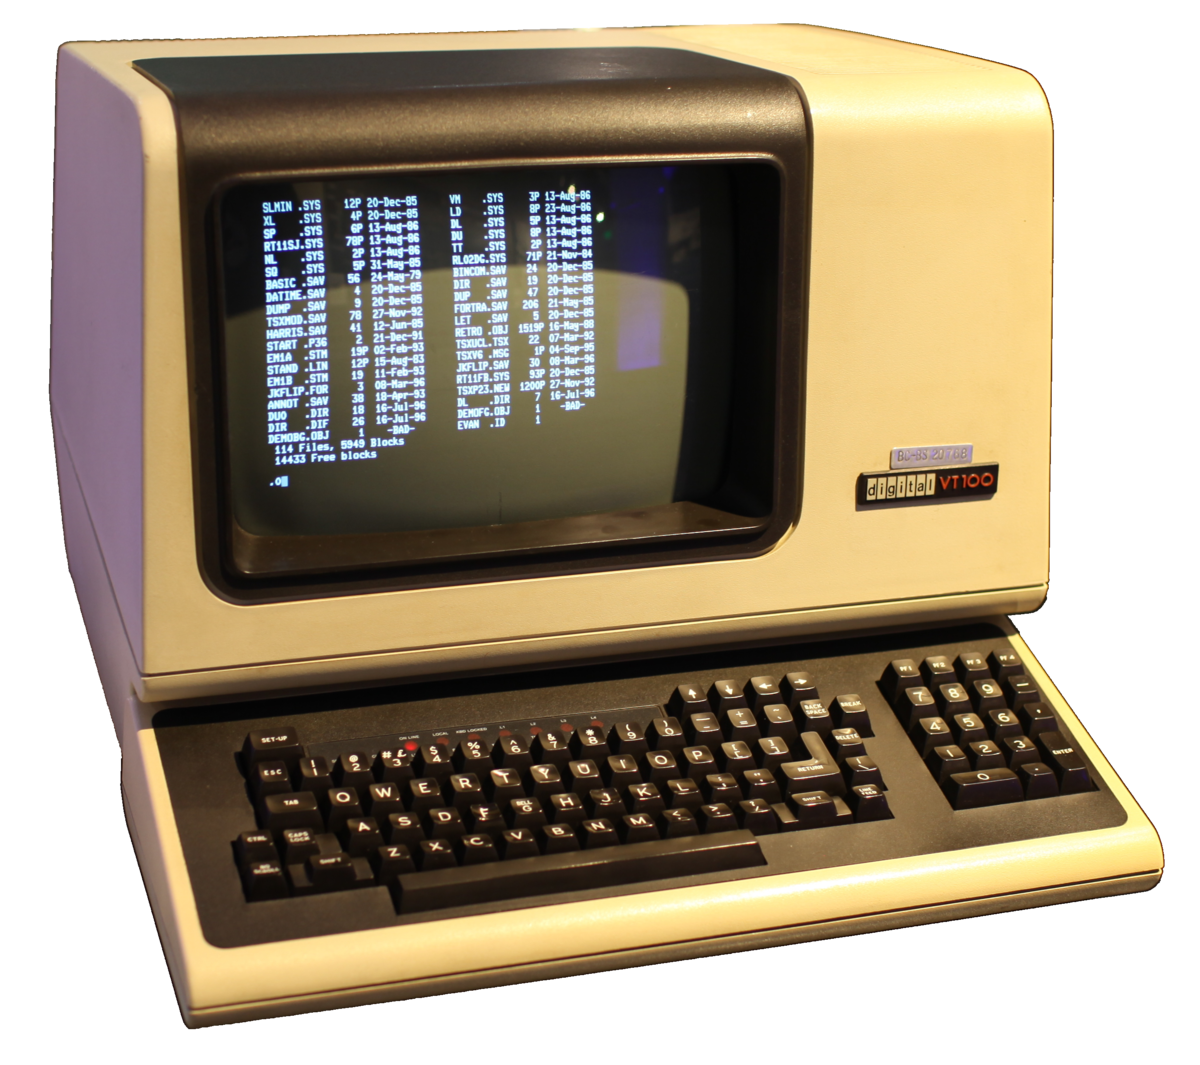
\includegraphics[width=0.9\textwidth]{terminal.png}
    \vspace{0.5em}\\
    {\small (Vintage terminál s textovým výstupem)}
  \end{columns}
\end{frame}


\section{Nela a medúzy}
\begin{frame}{Nela - adresář}
  \begin{itemize}
    \item Archiv budeme používat k naučení se základní navigace
    \item Stáhni archiv \texttt{data-shell.zip} z:
    \url{https://naucse.python.cz/2025/brno-podzim-linuxadmin/carpentry-unix/bash-intro/static/data-shell.zip}
    \item Ulož ho do adresáře \texttt{Dokumenty}
    \item Extrahuj data z archivu buď přes aplikaci Soubory, nebo zadej příkazy do terminálu:
  \end{itemize}

    \vspace{0.5em}
	{\ttfamily\small
		\$ cd Dokumenty \\
		\$ unzip data-shell.zip \\
		\$ cd \\
	}

\end{frame}


  \section{Navigace v souborech a adresářích}
  \begin{frame}{Navigace – základní příkazy}
    \begin{itemize}
      \item \texttt{pwd} – vypíše aktuální pracovní adresář
      \item \texttt{ls} – seznam souborů a složek
      \item \texttt{cd <cesta>} – změna adresáře
          \vspace{0.5em}
      \item Speciální symboly:
        \begin{itemize}
          \item \texttt{.} – aktuální adresář
          \item \texttt{..} – nadřazený adresář
          \item \texttt{\ts} – domovský adresář
          \item \texttt{/} – kořenový adresář
        \end{itemize}
            \vspace{0.5em}
      \item Relativní vs. Absolutní cesty
    \end{itemize}
  \end{frame}

\begin{frame}{Nápověda k příkazům}
  \begin{itemize}
    \item Většina příkazů má přepínač \texttt{-{}-help}:
    \begin{semiverbatim}
ls -{}-help
    \end{semiverbatim}
    \item Manuál příkazu lze zobrazit pomocí \texttt{man}:
    \begin{semiverbatim}
man ls
    \end{semiverbatim}
  \end{itemize}

\small
\texttt{Použití: ls [PŘEPÍNAČ]... [SOUBOR]...}\\
\texttt{Vypisuje informace o SOUBORECH (implicitně z aktuálního adresáře).}\\
\texttt{Jestliže není zadán žádný z přepínačů -cftuvSUX nebo -{}-sort,}
\texttt{výstup bude seřazen abecedně.}\\[0.5em]
\texttt{-a, -{}-all} \hspace{1em} \texttt{vypíše i soubory začínající tečkou}\\
\texttt{-A, -{}-almost-all} \hspace{1em} \texttt{vypíše všechny soubory kromě "." a ".."}\\
\hspace{1em} \texttt{-{}-author} \hspace{1em} \texttt{spolu s -l vypíše autora každého souboru}
\end{frame}

\section{Práce se soubory a adresáři}
    \begin{frame}{Pojmenování souborů}
        \begin{itemize}
          \item Nepoužívej mezery.
          \item Ideálně používej jen anglická písmenka, číslice, \texttt{.}, \texttt{-} a \texttt{\_}.
          \item Nezačínej pomlčkou \texttt{-}.
          \item Vyhni se diakritice.
          \item Drž se malých písmen.
          \item Tečku používej na oddělení přípony.
        \end{itemize}

            \vspace{1.5em}
    \textbf{Příklad dobrého pojmenování:} \texttt{data\_2025-09-30.csv} \\
    \textbf{Příklad nevhodného pojmenování:} \texttt{-moje.data!!!}
\end{frame}

  \begin{frame}{Práce se soubory a adresáři}
    \begin{itemize}
      \item \texttt{mkdir <dir>} – vytvořit adresář
      \item \texttt{touch <soubor>} – vytvořit prázdný soubor
      \item \texttt{cp <zdroj> <cíl>} – kopírovat
      \item \texttt{mv <zdroj> <cíl>} – přesunout / přejmenovat
      \item \texttt{rm <soubory>} – smazat
    \end{itemize}
  \end{frame}

\begin{frame}{Samostatná práce – Navigace}
\small
\textbf{Cíl:} Procvičit navigaci v adresářích a práci s cestami.\\[0.5em]

\textbf{Úkoly:}
\begin{enumerate}
  \item Zobraz svůj aktuální pracovní adresář (\texttt{pwd}).
  \item Přesuň se do složky \texttt{data-shell} pomocí relativní cesty (\texttt{cd}).
  \item Zobraz seznam souborů a složek (\texttt{ls}).
  \item Přesuň se do podsložky \texttt{data} a poté zpět do nadřazeného adresáře.
  \item Přesuň se do domovského adresáře (\texttt{\ts}) a poté do kořenového adresáře (\texttt{/}).
  \item Procvič relativní a absolutní cesty – ukaž, že oba způsoby vedou ke složce \texttt{data-shell/creatures}.
\end{enumerate}
\end{frame}

\begin{frame}{Samostatná práce – Základní příkazy pro soubory}
\small
\textbf{Cíl:} Procvičit vytváření souborů a adresářů a základní manipulaci.\\[0.5em]

\textbf{Úkoly:}
\begin{enumerate}
  \item Vytvoř novou složku \texttt{testdir} ve složce \texttt{data-shell}.
  \item Vytvoř prázdný soubor \texttt{novy.txt} uvnitř \texttt{testdir} (\texttt{touch}).
  \item Zkopíruj soubor \texttt{amino-acids.txt} ze složky \texttt{data} do \texttt{testdir} (\texttt{cp}).
  \item Přesuň soubor \texttt{data/animals.txt} do složky \texttt{testdir} (\texttt{mv}).
  \item Smaž soubor \texttt{novy.txt} (\texttt{rm}).
\end{enumerate}
\end{frame}

\begin{frame}{Samostatná práce – Nápověda a objevování}
\small
\textbf{Cíl:} Procvičit nápovědu a manuál k příkazům.\\[0.5em]

\textbf{Úkoly:}
\begin{enumerate}
  \item Zjisti, jak se používá příkaz \texttt{ls} pomocí \texttt{-{}-help}.
  \item Najdi přepínač pomocí kterého zobrazíš i velikost souborů.
  \item Zjisti, jak se používá příkaz \texttt{cd} pomocí \texttt{man}.

\end{enumerate}
\end{frame}


\section{Textový editor Vim}
\begin{frame}{Základy editoru Vim}
  \begin{itemize}
    \item Instalace Vimu: \texttt{sudo dnf install vim -y}

    \item \textbf{Editační mód (Normal mode)}
      \begin{itemize}
        \item Slouží k pohybu kurzoru a přesouvání částí textu, v tomto režimu
        nelze psát text
        \item Vstup do editačního módu: klávesa \texttt{Esc}
      \end{itemize}
            \vspace{0.5em}
    \item \textbf{INSERT mód}
      \begin{itemize}
        \item Slouží ke vkládání znaků do souboru
        \item Vstup do INSERT módu: klávesa \texttt{i}
        \item Ukončení INSERT módu: klávesa \texttt{Esc}
      \end{itemize}
            \vspace{0.5em}
    \item \textbf{Příkazový mód}
      \begin{itemize}
        \item Vim zobrazí vlastní příkazovou řádku, kam lze napsat příkaz
        \item Vstup do příkazového módu: klávesa \texttt{:}
        \item Ukončení příkazového módu: klávesa \texttt{Esc}
      \end{itemize}
            \vspace{0.5em}
    \item Uložení / ukončení: \texttt{:w}, \texttt{:q}, \texttt{:wq}, \texttt{:q!}
  \end{itemize}
\end{frame}

\begin{frame}{Samostatná práce – Vim}
\small
\textbf{Cíl:} Procvičit základní práci s Vimem: vytváření souboru, editace a ukládání.\\[0.5em]

\textbf{Úkoly:}
\begin{enumerate}
  \item Vytvoř prázdný soubor \texttt{vlastni.txt} a otevři ho ve Vimu:
  \begin{semiverbatim}
vim vlastni.txt
  \end{semiverbatim}
  \item Napiš do souboru nějaký text, ulož a ukonči.
  \item Otevři soubor znovu, přidej další řádek textu a ulož.
  \item Otevři soubor znovu, napiš něco, ale ukonči bez uložení.
\end{enumerate}

\textbf{Tipy:}
\begin{itemize}
  \item Přepni do INSERT módu klávesou \texttt{i} pro psaní textu.
  \item Přepni zpět do NORMAL módu klávesou \texttt{Esc}.
  \item Ulož a ukonči příkazem \texttt{:wq}, ukonči bez uložení \texttt{:q!}.
\end{itemize}
\end{frame}

  \section{Zkratky / užitečné klávesy}
  \begin{frame}{Zkratky}
    \begin{itemize}
      \item \texttt{AltGr+A} – tilda (\ts)
      \item \texttt{Tab} – automatické doplnění názvů
      \item \texttt{Ctrl+C} – ukončení příkazu
      \item \texttt{Ctrl+R} – hledání v historii
      \item \texttt{Ctrl+W} - smaže slovo před kurzorem
      \item \texttt{Ctrl} + šipky \texttt{←}, \texttt{→} - přesunují mezi slovy příkazu
      \item Šipky \texttt{↑}, \texttt{↓} – procházení historie
      \item \texttt{history} – výpis historie příkazů
    \end{itemize}
  \end{frame}


\end{document}
